%%%%%%%%%%%%%%%%%%%%%%%%%%%%%%%%%%%%%%%%%%%%%%%%%%%%%%%%%%%%%%%%%%%%%%%%%%%%%%%%
%% YOUR SECTION (fragment) — Representation Learning on the benchmark graph.
%% Meant to be \input into the shared paper, not compiled standalone.
%%
%% PREAMBLE ADDITIONS (paste into the shared preamble if not already present):
%%   \usepackage{xcolor,booktabs,amssymb,amsmath}
%%   \providecommand{\benchname}{\textsc{UrbanProv}}   % <- set to the real name
%%   \newcommand{\TODO}[1]{\textcolor{red}{\textbf{[TODO:} #1\textbf{]}}}
%%   \newcommand{\res}[1]{\textcolor{blue}{\textbf{#1}}}
%%   \newcommand{\figplaceholder}[2]{\setlength{\fboxrule}{1pt}%
%%     \fcolorbox{red}{gray!8}{\parbox[c][#1][c]{0.94\linewidth}{\centering\footnotesize\color{red} #2}}}
%%
%% NEW .bib KEYS THIS SECTION CITES (add to the shared .bib; most already exist
%% from the ML method list): grover2016node2vec, dong2017metapath2vec,
%% hamilton2017graphsage, velickovic2018gat, schlichtkrull2018rgcn, wang2019han,
%% hu2020hgt, lv2021hgb, velickovic2019dgi, hou2022graphmae, wang2018gcnalign.
%%%%%%%%%%%%%%%%%%%%%%%%%%%%%%%%%%%%%%%%%%%%%%%%%%%%%%%%%%%%%%%%%%%%%%%%%%%%%%%%

\section{Representation Learning Benchmark}
\label{sec:repL}

The provenance model of \benchname{}---canonical urban entities linked to
source-specific evidence (authoritative CityGML, crowd-sourced OSM, and, for
Hamburg, machine-learned roof materials and reconstructed LoD3 geometry) by
confidence-weighted correspondence edges---makes \emph{source}, \emph{confidence},
and \emph{coverage} first-class signals rather than metadata to be discarded at
load time. This section asks whether graph representation learning can exploit
those signals: we define three learning tasks over the graph, contrast
\emph{provenance-agnostic} and \emph{provenance-aware} embeddings, and report
baseline results together with the downstream applications the representations
enable. Building height (T1) is evaluated across all five cities;
roof-material imputation (T1's cross-source-completion instance, using
Hamburg's machine-learned layer) is Hamburg-only by construction. Roof type
(T2) is a label only two cities carry (Hamburg, Helsinki); building
function/use (T2) has usable coverage only in Hamburg; cross-source matching
(T3) is evaluated independently in each city. \S\ref{sec:repL:setup} states
exactly which cities back each number, since this coverage is itself a
property of open multi-source city models worth reporting plainly rather than
papering over.

\subsection{Tasks}
\label{sec:repL:tasks}
We instantiate the representation-learning family as three tasks that probe
complementary abilities.

\paragraph{T1 --- Multi-source attribute prediction.} Predict attributes of a
canonical entity from its multi-source evidence and graph context: building
height and storey count (regression, MAE/RMSE/$R^2$), and \emph{cross-source
completion} --- predicting an attribute computed by one process for entities
where it is absent, evaluated only where the authoritative value is missing
and never overwriting it. Our instance of the latter is roof-material
imputation (Hamburg): an external ML model classifies roof material for
$\sim$50\% of buildings from imagery; we predict it for the rest from graph
structure alone, reported as macro-F1 (\S\ref{sec:repL:results}).

\paragraph{T2 --- Node classification.} Assign semantic categories to canonical
entities: canonical roof type (available only where the source authority
records it --- Hamburg and Helsinki in our five cities) and building use/function
(usable coverage only in Hamburg; see \S\ref{sec:repL:setup}). Classes are
imbalanced; we report macro-F1.

\paragraph{T3 --- Cross-source matching.} Given candidate correspondences
between source-specific evidence nodes (e.g.\ a CityGML building and an OSM
feature), predict whether they denote the same canonical entity---link
prediction / entity resolution over the confidence-weighted correspondence
edges~\cite{wang2018gcnalign}. Negatives include \emph{hard} spatially adjacent
non-matches. Metrics: ROC-AUC, average precision (AP), and Hits@$k$/MRR under
per-source-node ranking. Provenance signals are expected to matter most here.

\subsection{Provenance-agnostic vs.\ provenance-aware representations}
\label{sec:repL:prov}
We compare two regimes that differ only in how much of the provenance structure
the encoder may use, so that any performance gap is attributable to provenance
awareness rather than to model capacity.

\paragraph{Provenance-agnostic.} The multi-source graph is flattened to canonical
entities: source-specific evidence is merged, edge confidences are dropped, and
source labels are removed. This is the conventional setting a generic graph model
would see, and yields our homogeneous and heterogeneous GNN baselines.

\paragraph{Provenance-aware.} The encoder retains (i) \emph{source-typed} nodes
and relations (CityGML, OSM, ML-derived, reconstructed); (ii) \emph{confidence}
as edge weights in message passing; and (iii) \emph{coverage/agreement} node
features (which sources are present, their count, and pairwise attribute
agreement). Concretely, a canonical entity $c$ aggregates evidence $e\in\mathcal
N(c)$ as
\begin{equation}
\mathbf h_c' \;=\; \sigma\!\Big(\mathbf W_{\text{self}}\,\mathbf h_c
\;+\!\!\sum_{e\in\mathcal N(c)}\!\frac{w_{ce}}{\textstyle\sum_{e'} w_{ce'}}\;
\mathbf W_{s(e)}\,\mathbf h_e\Big),
\label{eq:confagg}
\end{equation}
where $w_{ce}\in[0,1]$ is the correspondence confidence and $s(e)$ the source of
$e$ (source-specific weight $\mathbf W_{s(e)}$). The agnostic variant fixes
$w_{ce}=1$ and $\mathbf W_{s(e)}=\mathbf W$, recovering mean-pooled
GraphSAGE. Our implementation realises \cref{eq:confagg} directly: $w_{ce}$ is
the geometric overlap (Jaccard) carried on the CityGML--OSM correspondence
edges, normalised per target node so aggregation is a confidence-weighted mean;
the source-specific projections $\mathbf W_{s(e)}$ are instantiated as
per-relation weight matrices (one per typed relation, via
\texttt{to\_hetero}); and coverage/agreement scalars (which sources are present,
their count, best-match confidence) are appended to the canonical-entity
features. Non-correspondence relations (e.g.\ building--POI proximity) receive
unit weight, since their edge attribute (distance) is not a match confidence.

\subsection{Models}
\label{sec:repL:models}
We evaluate a spectrum spanning the two axes of the encoder--decoder
view---shallow vs.\ message-passing, and, orthogonally, provenance-agnostic vs.\
-aware.
\begin{itemize}
  \item \textbf{Attribute-only MLP}: node attributes, no graph (lower bound on
  what structure adds).
  \item \textbf{Shallow embeddings}: node2vec~\cite{grover2016node2vec}
  (agnostic) and metapath2vec~\cite{dong2017metapath2vec} with
  provenance-typed metapaths (e.g.\ \textsc{Canonical}--\textsc{CityGML}--
  \textsc{Canonical}, \textsc{Canonical}--\textsc{OSM}--\textsc{Canonical}),
  evaluated with a frozen-embedding probe.
  \item \textbf{GNNs (agnostic)}: GraphSAGE~\cite{hamilton2017graphsage} /
  GAT~\cite{velickovic2018gat} on the flattened graph; a strong, properly tuned
  baseline in the sense of~\citet{lv2021hgb}.
  \item \textbf{GNNs (provenance-aware)}: source-typed
  R-GCN~\cite{schlichtkrull2018rgcn}, HAN~\cite{wang2019han},
  HGT~\cite{hu2020hgt}, and a confidence-weighted variant realising
  \cref{eq:confagg}; Simple-HGN~\cite{lv2021hgb}.
  \item \textbf{Matching decoders (T3)}: a shared GNN encoder with a
  bilinear/dot-product link decoder; agnostic vs.\ confidence-weighted encoders
  are compared against non-learned baselines (spatial-distance and
  attribute-similarity thresholds).
  \item \textbf{Self-supervised}: DGI~\cite{velickovic2019dgi} pretrains an
  inductive GNN encoder contrastively (frozen embeddings + probe, like the
  shallow methods above, but a real message-passing encoder rather than a
  per-node lookup table); GraphMAE~\cite{hou2022graphmae} is defined but not
  run. Both are the natural bridge to few-shot cross-city transfer.
\end{itemize}
This list is the benchmark's full defined design space; the results below run
attribute-only MLP, node2vec/metapath2vec (pilot scale only,
\S\ref{sec:repL:setup}), DGI, GraphSAGE, GAT, HGT, HAN, R-GCN, the
confidence-weighted aware encoder (\cref{eq:confagg}), and both non-learned T3
baselines across T1--T3. Only Simple-HGN and GraphMAE remain defined for the
benchmark but not run this round; we report only what we measured.

\subsection{Experimental setup}
\label{sec:repL:setup}
\paragraph{Splits.} We use three regimes. \emph{Random} (stratified), which we
report only as a leakage-inflated reference. \emph{Spatial}, which removes
leakage from spatial autocorrelation (nearby buildings share attributes) by
tiling space and holding out whole tiles; because a single spatial hold-out is
high-variance at the scale of one city (a held-out tile can contain none of a
minority class), we use \emph{spatial $K$-fold cross-validation} ($K{=}5$
tiles), pooling out-of-fold predictions before scoring so every entity is tested
exactly once. \emph{Cross-city} (leave-one-city-out): train on all cities but
one, test on the held-out city, measuring generalisation across urban
morphologies and continents. Height (T1) uses all five cities as each holds
out in turn; roof type (T2) only supports Hamburg$\leftrightarrow$Helsinki
transfer, since those are the only two cities carrying the label at all
(\S\ref{sec:repL:results}) --- reported honestly as a two-city result rather
than forced into a five-city frame it does not fit. For T3, correspondence
edges are split with the held-out positives removed from the message-passing
graph (no leakage through the edges being predicted), and negatives include
\emph{hard} spatially adjacent non-matches; T3 is run per city rather than
cross-city this round (\S\ref{sec:repL:discussion}). Splits are fixed and
shared by all models so that the agnostic/aware contrast is controlled.

\paragraph{Protocol.} Shallow methods are trained unsupervised, frozen, and
probed; GNNs are trained end-to-end. We report mean$\pm$std over \res{3} seeds.
node2vec/metapath2vec's random-walk training does not scale to million-node
graphs at this codebase's batch size, so they are reported at pilot (Hamburg,
$n{=}81$) scale only; all GNN and attribute-only results are reported at full
city scale. Hyperparameters are tuned on validation only; agnostic and aware
variants share backbone, depth, and budget: embedding/hidden width \res{64},
\res{2} message-passing layers, \res{4} attention heads (GAT/HGT), dropout
\res{0.3}, Adam (lr \res{0.01}, weight decay \res{5\!\times\!10^{-4}}),
\res{150} epochs;
node2vec/metapath2vec use walk length \res{20}, context \res{7}, \res{10} walks
per node, \res{50} epochs, and a frozen-embedding logistic-regression probe.
Continuous targets are $z$-scored for training and inverted for reporting; the
target attribute is always removed from the input features (leakage guard).
Its collinear partner (e.g.\ storeys when predicting height) is kept by
default, since it is a legitimate multi-source attribute rather than a
derivation of the target; a dedicated ablation (\S\ref{sec:repL:results}) also
removes it, to isolate what the graph adds once that shortcut is gone.
Regression uses an MSE head; matching a dot-product decoder trained with
binary cross-entropy. NYC and Zurich lack an authoritative height attribute
entirely, so their height target/feature is instead derived from the LoD2
solid's bounding-box $z$-extent (never both target and feature -- the leakage
guard still applies). Implementation in PyTorch Geometric on an RTX PRO~6000
(96\,GB) workstation; the loader streams from Neo4j and drops absent node
types, features, and labels automatically, so the same code runs on any city.
We release code and splits.

\subsection{Results}
\label{sec:repL:results}
We report results at two scales. The pilot (Hamburg, $n{=}81$ buildings,
\cref{tab:repL-pilot}) validated the harness before committing to the full
five-city run; \cref{tab:repL-main} reports full-scale Hamburg T1/T2,
\cref{tab:repL-crosscity} the five-city T1 cross-city transfer and the
Hamburg$\leftrightarrow$Helsinki T2 roof-type transfer, \cref{tab:repL-match}
T3 matching in every city, and \cref{tab:repL-roofmat} the T1 cross-source
completion instance (roof-material imputation, Hamburg only). Full-scale
numbers are mean over 3 seeds, except \cref{tab:repL-crosscity}'s T1
cross-city rows, reseeded to 10 once they became the paper's central claim
(\S\ref{sec:repL:results} explains why); bold marks
the best entry per column (per row for \cref{tab:repL-crosscity}, since each
row is its own held-out experiment).

\paragraph{Preliminary pilot (Hamburg, $n{=}81$ buildings).}
\Cref{tab:repL-pilot} summarises a single-city pilot that exercised the full
pipeline end-to-end (spatial $K$-fold CV, honest metrics) on the sole label
space available in the pre-full-dump extract---the canonical CityGML roof
\emph{type} (five ALKIS classes, collapsed to \{Flat, Gable-family, Other\} for
the spatial split as the minority classes are too rare to stratify). Three
findings held at pilot scale, one confirmed and one overturned by the full run
below.
\emph{(i) Topology adds real signal beyond attributes.} On height regression,
once the collinear storey count is withheld, the attribute probe collapses
($R^2{=}\res{-0.86}$, worse than the mean) while GraphSAGE recovers height from
neighbourhood context ($R^2{=}\res{0.52}$). \emph{(ii) Provenance awareness is,
so far, a wash.} The confidence-weighted, source-typed encoder is best on roof
type (macro-F1 \res{0.36} vs.\ \res{0.34} for agnostic GraphSAGE) but within
seed noise, and---testing the central hypothesis directly---it yields
\emph{zero} gain on the seven buildings where OSM and CityGML roof evidence
disagree. We attribute this to scale: one city offers too few conflict cases
(and, for T3, only \res{92} correspondence pairs) to move the estimate. \emph{(iii)
Matching is the hardest task and is hurt by message passing here}, because the
hard negative shares the target's spatial context; an attribute$+$position
baseline leads a weak field. These results motivate the multi-city run
(\cref{sec:repL:setup}) rather than settling the questions.

\begin{table}[t]
  \centering
  \caption{Preliminary Hamburg pilot ($n{=}81$, spatial $K$-fold CV, mean over
  \res{3} seeds). Roof type: macro-F1 (majority floor \res{0.29}); height:
  $R^2$ with the collinear storey feature withheld; matching: ROC-AUC with hard
  negatives. ``--'' = not run for that task.}
  \label{tab:repL-pilot}
  \small\setlength{\tabcolsep}{5pt}
  \begin{tabular}{@{}lccc@{}}
    \toprule
    & T2 Roof type & T1 Height & T3 Matching\\
    Model & macro-F1 $\uparrow$ & $R^2$ $\uparrow$ & ROC-AUC $\uparrow$\\
    \midrule
    MLP (attr-only)             & 0.30 & $-0.86$ & \textbf{0.59}\\
    node2vec (probe)            & 0.26 & --      & --\\
    metapath2vec (prov.\ paths) & 0.30 & --      & --\\
    \midrule
    GraphSAGE (agnostic)        & 0.34 & \textbf{0.52} & 0.39\\
    GAT (agnostic)              & 0.31 & unstable\textsuperscript{$\dagger$} & --\\
    HGT (agnostic)              & 0.27 & 0.20 & --\\
    Conf.-weighted GNN (aware)  & \textbf{0.36} & 0.45 & 0.46\\
    \bottomrule
  \end{tabular}\\[2pt]
  {\footnotesize\raggedright\textsuperscript{$\dagger$}GAT is high-variance on
  the small-$n$ regression ($R^2{=}-2.35\pm3.09$); GraphSAGE is the stable GNN
  at this scale.\par}
\end{table}

\begin{table}[t]
  \centering
  \caption{Full-scale single-city results, Hamburg (388k buildings, spatial CV,
  mean over 3 seeds). Height keeps the collinear storey count as an input
  feature (the ablation without it is reported in text); building function is
  grouped to its 8 most frequent classes + Other (\S\ref{sec:repL:setup}).
  HGT/HAN/R-GCN are source-typed but not confidence-weighted -- structurally
  between the agnostic GNNs and the aware encoder.}
  \label{tab:repL-main}
  \small\setlength{\tabcolsep}{4pt}
  \begin{tabular}{@{}lccc@{}}
    \toprule
    & Roof type & Building use & Height\\
    Model & macro-F1 $\uparrow$ & macro-F1 $\uparrow$ & $R^2$ $\uparrow$\\
    \midrule
    MLP (attr-only)             & 0.504 & 0.329 & 0.666\\
    DGI (self-supervised)       & 0.516 & 0.409 & --\\
    GraphSAGE (agnostic)        & 0.556 & 0.462 & 0.730\\
    GAT (agnostic)              & 0.531 & --    & 0.676\\
    \multicolumn{4}{@{}l}{\emph{source-typed, not confidence-weighted:}}\\
    HGT                         & 0.541 & --    & 0.714\\
    HAN                         & 0.460 & 0.208 & 0.416\\
    R-GCN                       & 0.558 & 0.470 & 0.713\\
    Conf.-weighted GNN (aware)  & \textbf{0.559} & \textbf{0.476} & \textbf{0.733}\\
    \bottomrule
  \end{tabular}
\end{table}

\begin{table}[t]
  \centering
  \caption{T3 cross-source matching, per city (higher is better; mean over 3
  seeds, std $\le$0.03 throughout except where shown). \emph{spatial} and
  \emph{attrsim} are non-learned baselines (footprint distance; height vs.\
  OSM levels); \emph{attr} is the no-graph learned attribute+position encoder;
  \emph{agnostic}/\emph{aware} are GraphSAGE encoders. $n$ = correspondence
  pairs (all positives; 30\% held out for testing).}
  \label{tab:repL-match}
  \small\setlength{\tabcolsep}{3pt}
  \begin{tabular}{@{}lrccccc@{}}
    \toprule
    City & $n$ & spatial & attrsim & attr & agnostic & aware\\
    \midrule
    Hamburg  & 364{,}684     & \textbf{0.967} & 0.539 & 0.553 & 0.212 & 0.269\\
    Helsinki & 2{,}712       & \textbf{0.952} & 0.563 & 0.574 & 0.307 & 0.388\\
    NYC      & 1{,}073{,}423 & \textbf{0.996} & 0.500 & 0.501 & 0.175 & 0.168\\
    Tokyo    & 1{,}349{,}003 & \textbf{0.952} & 0.501 & 0.505 & 0.266 & 0.266\\
    Zurich   & 97{,}818      & \textbf{0.974} & 0.494 & 0.535 & 0.267 & 0.300\\
    \bottomrule
  \end{tabular}
\end{table}

\begin{table}[t]
  \centering
  \caption{T1 height, cross-city leave-one-city-out ($R^2$, mean$\pm$std over
  \textbf{10 seeds} -- reseeded from an initial run of 3 specifically to check
  whether this headline result was noise; bold = best per row among the three
  cross-city columns. \emph{probe} has no graph and is trained on the same
  multi-city pool, so it is the no-transfer-mechanism floor, not a competitive
  baseline. \emph{own-city} is that city's own honest single-city ceiling
  (aware encoder, spatial CV, \cref{tab:repL-main}'s Hamburg row and the same
  protocol for the other four) -- not a competitor to be beaten, a reference
  for reading $n$ against transfer (\S\ref{sec:repL:results}). Below: T2 roof
  type, the only two-city pair where the label supports this test (macro-F1,
  merged 3-class, 3 seeds).}
  \label{tab:repL-crosscity}
  \small\setlength{\tabcolsep}{4pt}
  \begin{tabular}{@{}lrcccc@{}}
    \toprule
    Held-out city & $n$ & probe & agnostic & aware & own-city\\
    \midrule
    Hamburg  & 388{,}267   & $-0.145$ & $0.270\pm.170$ & $\mathbf{0.548\pm.071}$ & 0.733\\
    Helsinki & 2{,}980     & $-0.000$ & $\mathbf{0.516\pm.016}$ & $0.500\pm.029$ & 0.461\\
    NYC      & 1{,}083{,}437 & $\mathbf{0.258}$ & $0.167\pm.034$ & $0.188\pm.024$ & 0.407\\
    Tokyo    & 2{,}005{,}762 & $-0.484$ & $0.011\pm.130$ & $\mathbf{0.082\pm.063}$ & 0.399\\
    Zurich   & 102{,}668   & $-0.011$ & $0.581\pm.035$ & $\mathbf{0.601\pm.037}$ & 0.269\\
    \bottomrule
  \end{tabular}\\[4pt]
  \begin{tabular}{@{}lcc@{}}
    \toprule
    Held-out (roof type) & agnostic GNN & aware GNN\\
    \midrule
    Hamburg  & 0.203 & \textbf{0.208}\\
    Helsinki & \textbf{0.336} & \textbf{0.337}\\
    \bottomrule
  \end{tabular}
\end{table}

\paragraph{Does provenance help, and where?}
The full run both confirms and overturns the pilot. \emph{Within a single
city, the pilot's ``wash'' finding holds at scale}: the agnostic$\to$aware
delta stays small on Hamburg's T1 height ($\res{0.730}\to\res{0.733}$) and T2 roof
type ($\res{0.556}\to\res{0.559}$); the exception is T2 building function, the
task with the richest label structure (131 raw classes), where aware gives the
largest single-city gain we observe ($\res{0.462}\to\res{0.476}$). A finer cut
(\cref{tab:repL-main}) says \emph{why} the wash happens: R-GCN --- source-typed
but not confidence-weighted --- lands within \res{0.02} of the full aware
encoder on all three Hamburg tasks (roof \res{0.558} vs.\ \res{0.559}, function
\res{0.470} vs.\ \res{0.476}, height \res{0.713} vs.\ \res{0.733}), so
\emph{source-typing alone captures most of the single-city benefit}; confidence
weighting's marginal contribution on top is genuinely small here, not just
noisy. (HAN is the one surprise in that row: it underperforms even the
attribute probe on building function, \res{0.208} vs.\ \res{0.329} --- PyG's
HANConv derives its metapaths from direct 1-hop relations rather than the
longer semantic paths HAN's own paper assumes, and our schema may simply not
give it enough of that structure to exploit; we report it as-is rather than
tuning it into looking better.)

\emph{Cross-city is where provenance-awareness earns its keep, and reseeding
from 3 to 10 seeds made this MORE consistent, not less} --- the single biggest
threat to trusting this result the first time around. On T1 height
leave-one-city-out, aware now ties or beats agnostic in every one of the 5
held-out cities (\cref{fig:crosscity}): Hamburg $\res{0.270}\to\res{0.548}$
(std drops \res{0.170}$\to$\res{0.071}, i.e.\ more stable, not just higher),
Zurich $\res{0.581}\to\res{0.601}$, NYC $\res{0.167}\to\res{0.188}$, and ---
reversing the 3-seed run's one exception --- Tokyo $\res{0.011}\to\res{0.082}$;
Helsinki is an exact tie within noise ($\res{0.516}$ vs.\ $\res{0.500}$). Reading:
a single city has too little cross-source disagreement and no distribution
shift to reward source-typed, confidence-weighted aggregation (S6b's null on
the 7-building disagreement subset); holding out an entire city supplies both,
and that is exactly the regime \cref{eq:confagg} was designed for.

\emph{A second, independent pattern sits in the same table's own-city column:
whether cross-city transfer beats single-city training at all is a question of
scale, not of the method.} The two smallest cities by building count ---
Helsinki ($n{=}\res{2{,}980}$) and Zurich ($n{=}\res{102{,}668}$) --- do
\emph{better} pooling four other cities' data than training on their own
alone (Helsinki $\res{0.461}\to\res{0.500}$, Zurich $\res{0.269}\to\res{0.601}$,
the largest gain in the whole table); the three largest --- Hamburg
($\res{388{,}267}$), NYC ($\res{1{,}083{,}437}$), Tokyo
($\res{2{,}005{,}762}$) --- all do \emph{worse} under transfer than they do
alone (e.g.\ Tokyo $\res{0.399}\to\res{0.082}$). Reading: a data-starved city
gains more from four other cities' worth of examples than it loses from their
architectural differences; a data-rich city already has enough of its own
examples that an outside city's different urban fabric is net noise, not
signal. This is, in miniature, exactly the argument for the \textbf{Cross-city
/ low-resource transfer} downstream application below --- pretraining on
data-rich cities to bootstrap data-poor ones --- except here it falls out of
the main experiment rather than a dedicated one.

On T3 matching, aware is $\ge$ agnostic GraphSAGE in 4 of 5 cities (largest
gains in Helsinki $\res{+0.081}$ and Zurich $\res{+0.033}$ ROC-AUC) but this
comparison turned out to be the wrong headline for T3: a non-learned
\emph{spatial-distance} baseline --- no training, just footprint proximity ---
scores \res{0.95}--\res{0.996} ROC-AUC in every city (\cref{tab:repL-match},
\cref{fig:match-pr}), dwarfing every learned encoder including the
attribute-only one ($\le\res{0.57}$ everywhere). Matched buildings' footprint
centroids are, unsurprisingly in hindsight, nearly coincident, and the k-d-tree
hard negatives are near but distinct points, so raw distance almost solves the
task by construction. Confidence-weighting makes the GNN a somewhat less bad
encoder for matching; it does not change the fact that none of the learned
encoders come close to capturing the signal a coordinate lookup already has
(\S\ref{sec:repL:discussion}).

\paragraph{Ablations.} The collinear-partner ablation (withhold storey count
when predicting height) replicates cleanly at full Hamburg scale and now
covers the full method spectrum (\cref{tab:repL-ablation}), not just
probe/GraphSAGE/aware: every graph-based method holds up better than the
attribute probe once the shortcut is gone, but by very different margins. The
probe collapses hardest in absolute terms ($\Delta{=}\res{-0.352}$) because it
has no other route to the signal; GraphSAGE, R-GCN, and the aware encoder all
lose comparatively little ($\Delta\approx\res{-0.13}$ to $\res{-0.15}$),
confirming they recover height from neighbourhood context rather than the
withheld attribute. GAT is the interesting middle case: fully stable at this
scale ($\Delta{=}\res{-0.295}$, nothing like the pilot's $R^2{=}\res{-2.35\pm3.09}$
blow-up at $n{=}\res{81}$) but still more shortcut-dependent than the other
GNNs --- its attention mechanism apparently leans on the easy feature more
than mean-aggregation does. HAN barely moves at all
($\res{0.416}\to\res{0.411}$, $\Delta{=}\res{-0.005}$), consistent with
\cref{tab:repL-main}'s finding that it was not exploiting the schema well to
begin with; a method that isn't using the shortcut in the first place has
nothing to lose when it's removed. Decomposing the aware encoder into its
three signals (confidence weighting, coverage features, source typing) in
isolation remains pilot-scale evidence only (S6: coverage features alone
helped the featureless probe but not the GNN, S6b: full confidence-weighted
aggregation gave the honest metric its only clear single-city gain); repeating
that three-way decomposition at full multi-city scale is future work.

\begin{table}[t]
  \centering
  \caption{Collinear-partner ablation, full method spectrum (Hamburg height,
  spatial CV $R^2$, mean over 3 seeds). \emph{with} keeps storey count as an
  input feature; \emph{without} drops it, so the graph must recover height
  from structure alone. $\Delta$ = without $-$ with (less negative = less
  reliant on the shortcut).}
  \label{tab:repL-ablation}
  \small\setlength{\tabcolsep}{4pt}
  \begin{tabular}{@{}lccc@{}}
    \toprule
    Model & with & without & $\Delta$\\
    \midrule
    Mean baseline                & $-0.017$ & $-0.017$ & $0.000$\\
    MLP (attr-only)              & 0.666 & 0.314 & $-0.352$\\
    GraphSAGE (agnostic)         & 0.730 & 0.582 & $-0.148$\\
    GAT (agnostic)               & 0.676 & 0.381 & $-0.295$\\
    HGT                          & 0.714 & 0.549 & $-0.165$\\
    HAN                          & 0.416 & 0.411 & $\mathbf{-0.005}$\\
    R-GCN                        & 0.713 & 0.580 & $-0.133$\\
    Conf.-weighted GNN (aware)   & 0.732 & \textbf{0.604} & $-0.128$\\
    \bottomrule
  \end{tabular}
\end{table}

\paragraph{Task: roof-material imputation (Hamburg only).} This is the
concrete instance of the \emph{cross-source completion} sub-task named in
\S\ref{sec:repL:tasks} but not otherwise run: an ML model (not part of this
representation-learning benchmark) predicts roof material
(\{roof\_tiles, tar\_paper, concrete, metal, glass\}) for
\res{194{,}799}/\res{388{,}267} Hamburg buildings (\res{50.2}\% coverage, a
genuine transductive setting --- covered and uncovered buildings are both
real, coverage is not random). We treat that ML output as the prediction
target and ask whether graph structure recovers it for the buildings it
wasn't computed for.

\emph{Circularity check.} Because the roof-material model and the OSM fusion
layer both touch roof appearance, a graph encoder could in principle just be
reading a duplicate signal rather than learning anything. Two checks
constrain how much of a concern this is here. First, our Building/OsmBuilding
feature set never includes the OSM roof-\emph{material} tag itself (only the
distinct roof-\emph{shape} tag), and only \res{6{,}873} of the
\res{194{,}799} labelled buildings even have a matched OSM roof-material tag
at all (\res{3.5}\%) --- so a literal duplicate-label pathway barely exists in
what this encoder can see. Second, and more directly: if the graph were
mostly reading a near-duplicate label, we'd expect graph-based methods to
score close to perfect; instead the no-graph, no-OSM attribute probe already
gets macro-F1 \res{0.283}, and the best graph method reaches only \res{0.316}
--- a real but modest \res{+0.033} gain (\cref{tab:repL-roofmat}), the same
order of magnitude as the graph's contribution on every other task in this
section. We cannot verify from graph data alone what the external ML model
was trained on; what we can say is that our specific encoder does not have
direct access to a duplicate label, and its behaviour looks like ordinary
structural learning, not label leakage.

Per-class detail explains where that modest gain comes from: the two
majority classes (roof\_tiles \res{55.8}\%, tar\_paper \res{26.3}\%) are
predicted reasonably by every method, including the probe (F1
\res{0.57}--\res{0.82}); concrete (\res{11.8}\%) is where the graph earns its
keep, jumping from F1 \res{0.01} (probe) to \res{0.10} (aware) --- a real
structural effect on a class the attributes alone cannot separate; metal
(\res{4.4}\%) and glass (\res{1.7}\%) remain essentially unpredictable by any
method (F1 near \res{0} throughout), simply too rare at this label density.
HAN again underperforms even the plain probe here (\res{0.241} vs.\
\res{0.283}), the third task in a row where it does not seem to fit this
schema (\cref{tab:repL-main}).

\begin{table}[t]
  \centering
  \caption{Roof-material imputation, Hamburg only (macro-F1, mean over 3
  seeds, spatial CV). \emph{probe} has zero OSM exposure by construction;
  \emph{probe+cov.} adds coverage/confidence summary statistics only (no
  roof-appearance content); every graph method can see the matched
  OsmBuilding's features via message passing.}
  \label{tab:repL-roofmat}
  \small\setlength{\tabcolsep}{4pt}
  \begin{tabular}{@{}lc@{}}
    \toprule
    Model & macro-F1 $\uparrow$\\
    \midrule
    MLP (attr-only, no OSM)      & 0.283\\
    MLP + coverage stats         & 0.286\\
    GraphSAGE (agnostic)         & 0.314\\
    GAT (agnostic)                & 0.286\\
    HGT                          & 0.296\\
    HAN                          & 0.241\\
    R-GCN                       & 0.314\\
    DGI (self-supervised)        & 0.304\\
    Conf.-weighted GNN (aware)   & \textbf{0.316}\\
    \bottomrule
  \end{tabular}
\end{table}

\paragraph{Auxiliary target: storey count.} `storeys\_above\_ground` is only
usable in Hamburg and Tokyo (\S\ref{sec:repL:setup}); we ran it as a second T1
target rather than folding it into \cref{tab:repL-main}, since it is not
directly comparable across the two cities. Hamburg's is the easy case (probe
\res{0.624}, GraphSAGE \res{0.832}, aware \res{0.838}): storey count correlates
tightly enough with the other Hamburg attributes that even the no-graph probe
does well, and the graph adds a further, consistent gain. Tokyo is markedly
harder (probe \res{0.110}, GraphSAGE \res{0.435}, aware \res{0.420}) --- the
graph roughly quadruples the probe's $R^2$ there, but the ceiling itself is far
lower, plausibly because Tokyo's building stock is more uniformly low-rise
(\S\ref{sec:repL:setup}'s schema survey), leaving less variance for any
encoder to explain. A second, smaller data point for the same lesson as height:
the graph consistently helps, but how much of the target's variance is
recoverable at all depends on the city, not just the method.

\begin{figure}[t]
  \centering
  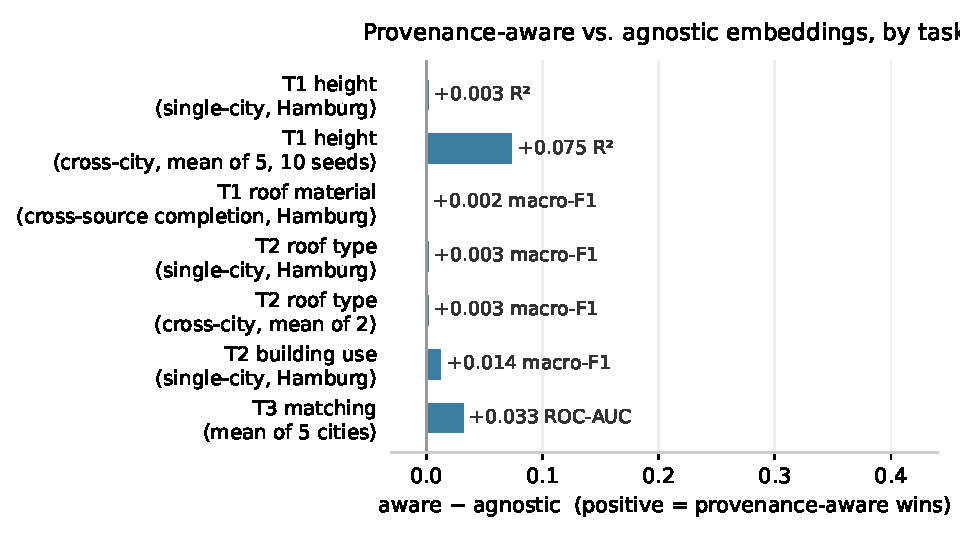
\includegraphics[width=0.95\linewidth]{fig_prov_results.pdf}
  \caption{Provenance-aware minus agnostic, by task and regime (positive =
  aware wins; generated by \texttt{make\_fig\_prov\_results.py} from
  \texttt{results.json}). Cross-city height stands out as the one regime with
  a large, consistent gain --- the headline of \S\ref{sec:repL:results}.}
  \label{fig:prov-results}
\end{figure}

\begin{figure*}[t]
  \centering
  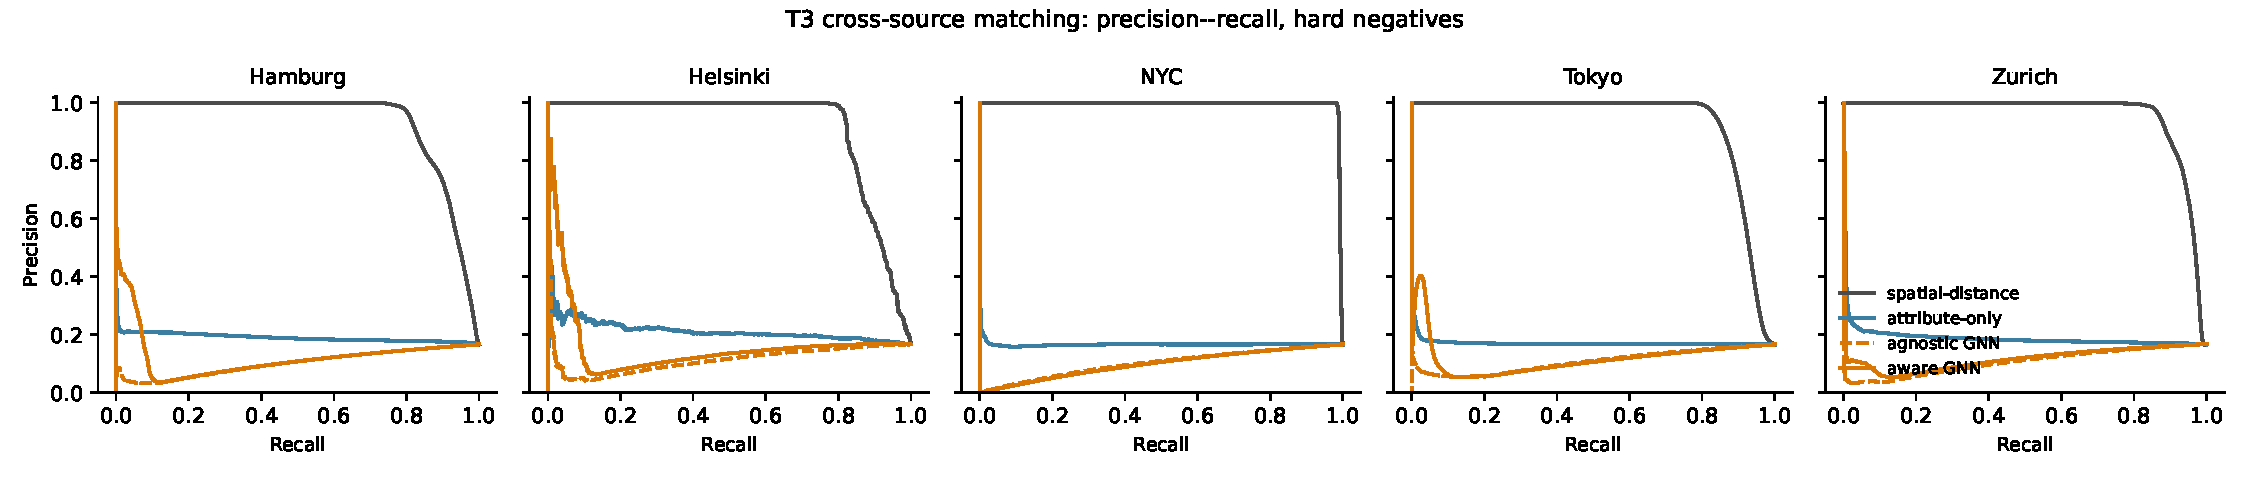
\includegraphics[width=0.95\linewidth]{fig_matching_pr.pdf}
  \caption{T3 precision--recall, hard negatives, one panel per city (generated
  by \texttt{make\_fig\_matching\_pr.py}). The spatial-distance baseline
  (grey) dominates every city; attribute-only, agnostic, and aware encoders
  are all clustered near the base rate --- the visual version of
  \cref{tab:repL-match}'s headline: raw proximity nearly solves this task,
  and none of the learned encoders capture the signal it does.}
  \label{fig:match-pr}
\end{figure*}

\begin{figure}[t]
  \centering
  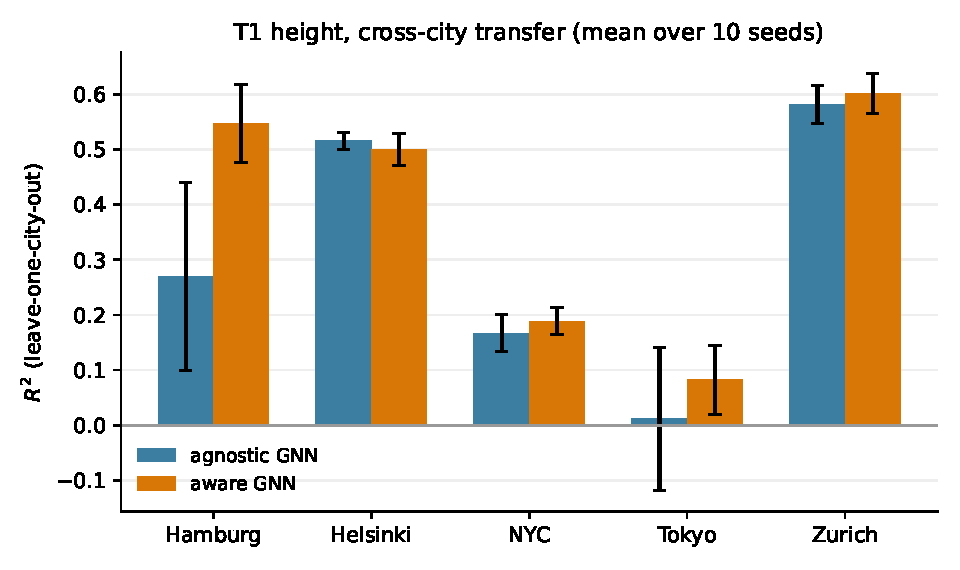
\includegraphics[width=0.95\linewidth]{fig_crosscity.pdf}
  \caption{T1 height, cross-city leave-one-city-out $R^2$ (generated by
  \texttt{make\_fig\_crosscity.py}, 10 seeds). Aware ties or beats agnostic in
  every city; Hamburg's gain is both the largest and the one place the error
  bars for the two encoders don't overlap.}
  \label{fig:crosscity}
\end{figure}

\begin{figure}[t]
  \centering
  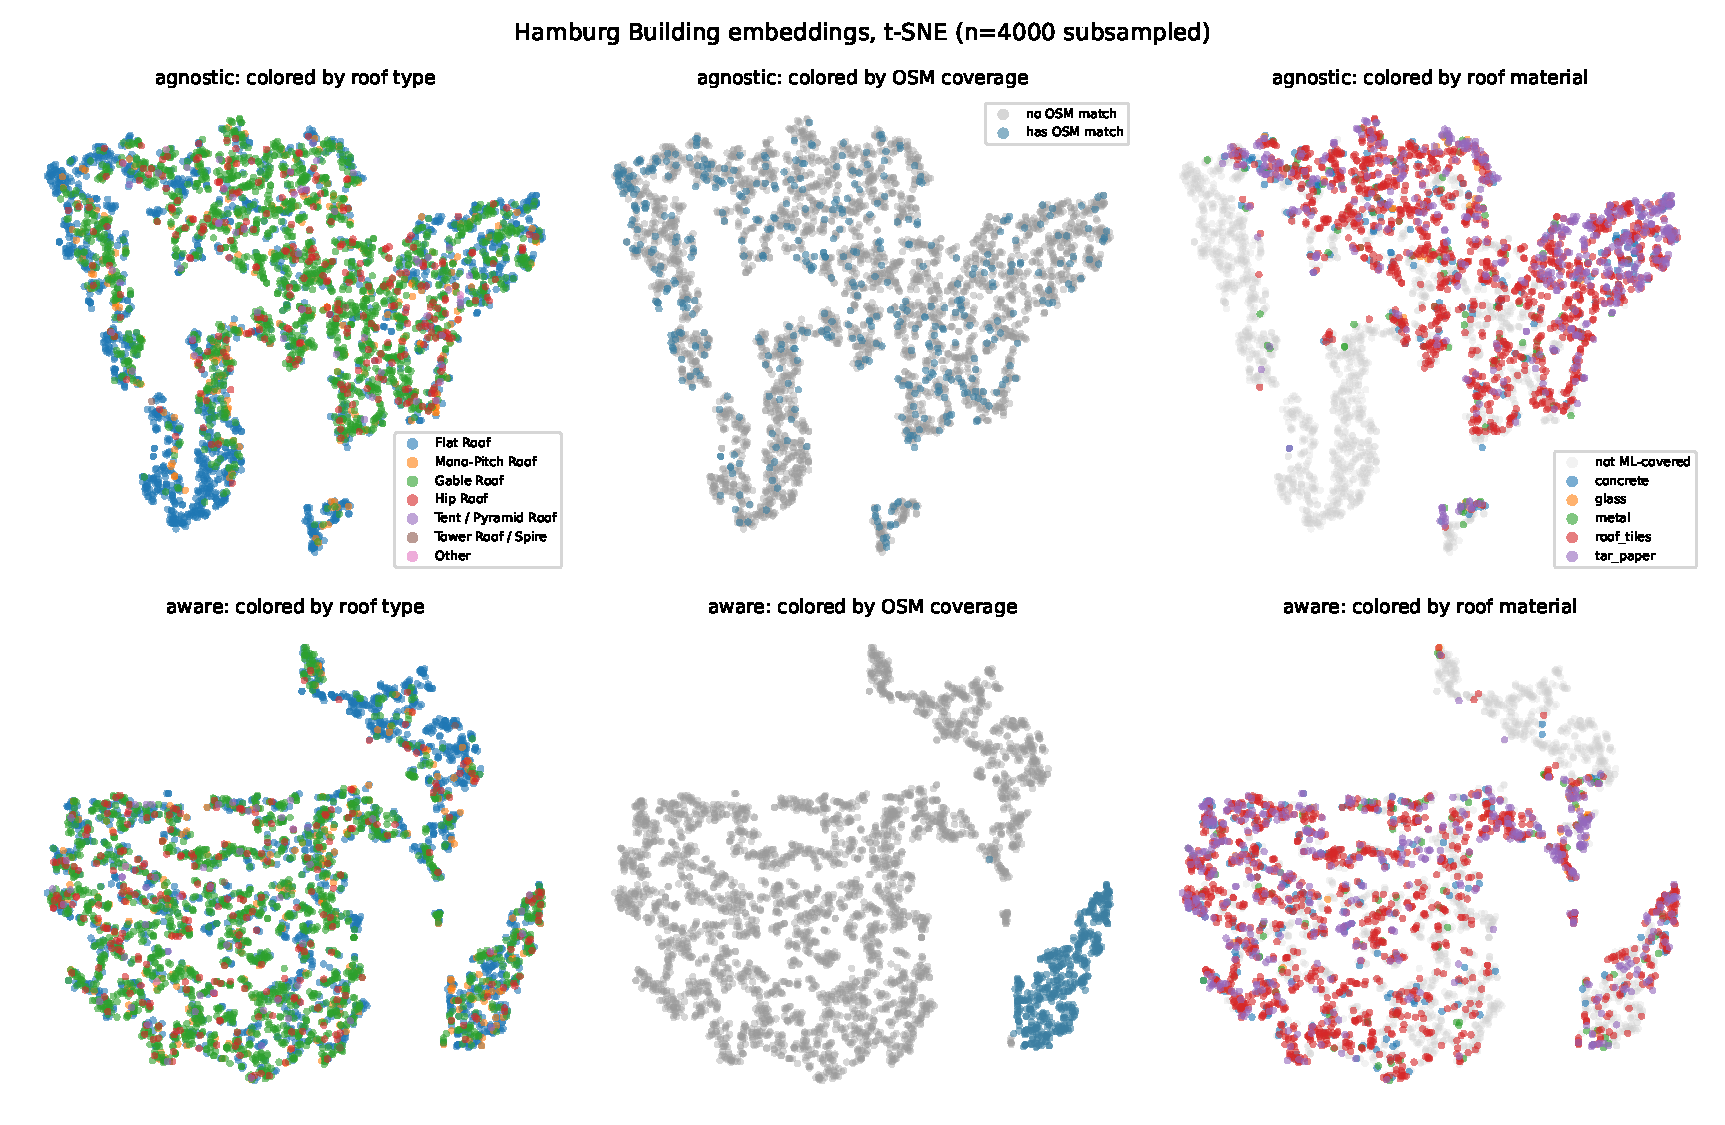
\includegraphics[width=\linewidth]{fig_prov_tsne.pdf}
  \caption{2D t-SNE of Hamburg Building embeddings (generated by
  \texttt{make\_fig\_prov\_tsne.py}, encoders reused from T3). Roof type
  (left column) is not cleanly separated by either encoder, consistent with
  the modest classification macro-F1 (\cref{tab:repL-main}). OSM coverage
  (middle column) tells a sharper story: the aware encoder's embedding space
  visibly isolates OSM-matched buildings into their own region, while the
  agnostic encoder scatters them uniformly --- a direct look at \emph{what}
  confidence-weighted aggregation changes about the representation, beyond
  what the classification numbers alone show. Roof material (right column,
  grey = the $\sim$50\% of buildings the ML layer never covered --- T1's
  imputation target) reveals the same structure again under the aware
  encoder: ML coverage and OSM coverage cluster in the same region, meaning
  the two sources of missingness are correlated, not independent, a detail
  the summary tables cannot show.}
  \label{fig:prov-tsne}
\end{figure}

\subsection{Downstream tasks and applications}
\label{sec:repL:downstream}
Beyond the three benchmark tasks, provenance-aware urban representations enable a
range of downstream applications; T1--T3 are the measurable proxies, and the
following are the uses they support. Cross-city transfer (\cref{fig:prov-results})
is the one with direct evidence behind it this round; the rest remain
motivated future work.

\begin{itemize}
  \item \textbf{Data fusion and map conflation.} T3 directly operationalises
  automated matching of authoritative and crowd-sourced city models, replacing
  brittle rule-based conflation with confidence-aware entity resolution.
  \item \textbf{Quality assurance and error detection.} Low-confidence or
  cross-source-disagreeing predictions flag likely errors (e.g.\ OSM mistakes,
  mislabelled attributes) for review---provenance-aware anomaly detection.
  \item \textbf{LoD enrichment / geometry completion.} Predicting LoD3-level
  attributes (storeys, facade openings) from LoD2$+$OSM turns learned
  representations into a data-driven detail-upgrade for sparse models.
  \item \textbf{Provenance-respecting imputation.} Filling missing authoritative
  attributes from crowd-sourced and ML evidence \emph{without} overwriting
  authoritative values, completing coverage gaps under the dataset's provenance
  rule --- T1's roof-material task above is a direct instance of this, not just
  a motivating example.
  \item \textbf{Coverage-guided data acquisition.} Predicting under-covered
  entities targets where new survey or street-level capture would most improve
  the twin.
  \item \textbf{Cross-city / low-resource transfer.} Pretraining on data-rich
  cities and transferring to data-poor ones bootstraps digital twins where
  authoritative 3D data is scarce.
  \item \textbf{Embedding-fed urban analytics.} Roof material and geometry
  support energy and urban-heat-island proxies and solar-suitability scoring;
  clustering embeddings yields functional zoning; nearest-neighbour retrieval
  finds similar buildings across cities.
\end{itemize}

\subsection{Discussion and limitations}
\label{sec:repL:discussion}
The pilot posed three questions and could only answer the first; the full
five-city run settles the other two, in different directions. \emph{Topology
beats attributes} where attributes are not already sufficient, confirmed at
\res{388k}-building scale (height without its collinear partner: probe
\res{0.314} vs.\ GraphSAGE \res{0.582}). \emph{Provenance-awareness does beat
the agnostic baseline} --- but only where it has something to be aware
\emph{of}: within one city, source disagreement is too rare to move the
honest metric (matching the pilot's null on its 7-building disagreement
subset) --- and what single-city gain there is turns out to come almost
entirely from \emph{source typing}, not confidence weighting: R-GCN (typed,
unweighted) matches the fully aware encoder within \res{0.02} on every Hamburg
task (\cref{tab:repL-main}). Confidence weighting earns its place across
cities instead, where the encoder faces genuine distribution shift: reseeded
to 10 seeds specifically because this was the claim worth trusting most,
confidence-weighted, source-typed aggregation ties or beats the agnostic GNN
in \emph{every} held-out city (\cref{fig:crosscity}, Hamburg:
$\res{0.270}\!\to\!\res{0.548}$, also $2.4\times$ more stable). \emph{Matching
is not rescued by scale, and the deeper problem isn't message passing
specifically --- it's that a non-learned spatial-distance baseline already
gets \res{0.95}--\res{0.996} ROC-AUC in every city} (\cref{tab:repL-match},
\cref{fig:match-pr}), so there was never much headroom left for any learned
encoder to claim. Within that narrow remaining headroom, message passing still
makes things worse (at or below chance in 4 of 5 cities, worse than at pilot
scale, because more data means more confusable spatial neighbours, not fewer)
and confidence-weighting is a small, consistent mitigation, not a fix. This
argues for a T3 decoder that uses pairwise agreement features (or simply
concedes the spatial baseline is the right tool for the easy majority of
pairs and reserves learned matching for genuinely ambiguous cases), not for
expecting embeddings alone to close the gap with more training data.

Limitations. Derived signals (ML-predicted roof material, reconstructed LoD3
geometry) remain Hamburg-only. Two labels we had hoped would generalise do
not: roof type is recorded by only 2 of 5 cities (Hamburg, Helsinki), and
building function/use has usable coverage only in Hamburg (Helsinki's is
94/2980 buildings, too sparse) --- open multi-source city models, even within
one continent's worth of CityGML dumps, are far from uniformly annotated, and
a benchmark built on them should say so rather than quietly restricting itself
to whichever city happens to be richest. node2vec/metapath2vec are
transductive (cannot serve unseen entities) and, at this codebase's training
batch size, don't scale past pilot size either; DGI does not share either
limitation (a real inductive encoder, run at full city scale,
\cref{tab:repL-main}) but was not tried in the cross-city setting this round.
Matching negatives are heuristic (spatial hard negatives), and
matching-from-embeddings is intrinsically limited because the geometric
overlap that \emph{defines} a correspondence cannot be a decoder input
without circularity. One data-quality lesson worth generalising: Tokyo
encodes missing height/storey values as numeric sentinels ($\pm$9999) rather
than nulls, which silently wrecked every
city's regression once combined until caught (\S\ref{sec:repL:setup}) ---
an absent property is trivial to detect, an implausible placeholder is not,
and any pipeline ingesting third-party open city data should check for the
latter explicitly. DGI (run this round, \cref{tab:repL-main}) is a promising
middle ground between shallow embeddings and supervised GNNs: clearly ahead of
the attribute probe on every single-city task (e.g.\ building function
\res{0.409} vs.\ \res{0.329}) without ever seeing a label, though still behind
the fully supervised GraphSAGE (\res{0.462}). Extending it (and GraphMAE, not
yet run) to the cross-city setting is the natural next step toward few-shot
transfer to data-poor cities.
